\chapter{Introduction}
\markboth{Introduction}{}

Biological systems are self-organized at various scales, from forests down to molecules. In particular, the origin of animal lifeforms occurs through embryonic development, where stem cells divide and differentiate to form the different tissues that will constitute the organism.



\section{Embryonic development and organoids}

During development, pluripotent stem cells (PSCs) initiate the process of cellular differentiation, eventually forming all the tissues in the adult animal. Advances in stem cell biology have enabled the generation of \textit{in vitro} models of morphogenesis from PSCs, forming organ-like structures called organoids \linebreak \parencite{Huch_2017} (see Fi\-gure \ref{fig:pic-organoids}). The emerging field of synthetic embryo\-logy has used the previous tools to investigate in a dish previously inaccessible processes that occur in embryos \parencite{Liu_2009,Serra_2019,Gritti_2021,Sullivan_2023}. 

\begin{figure}[ht]
    \centering
    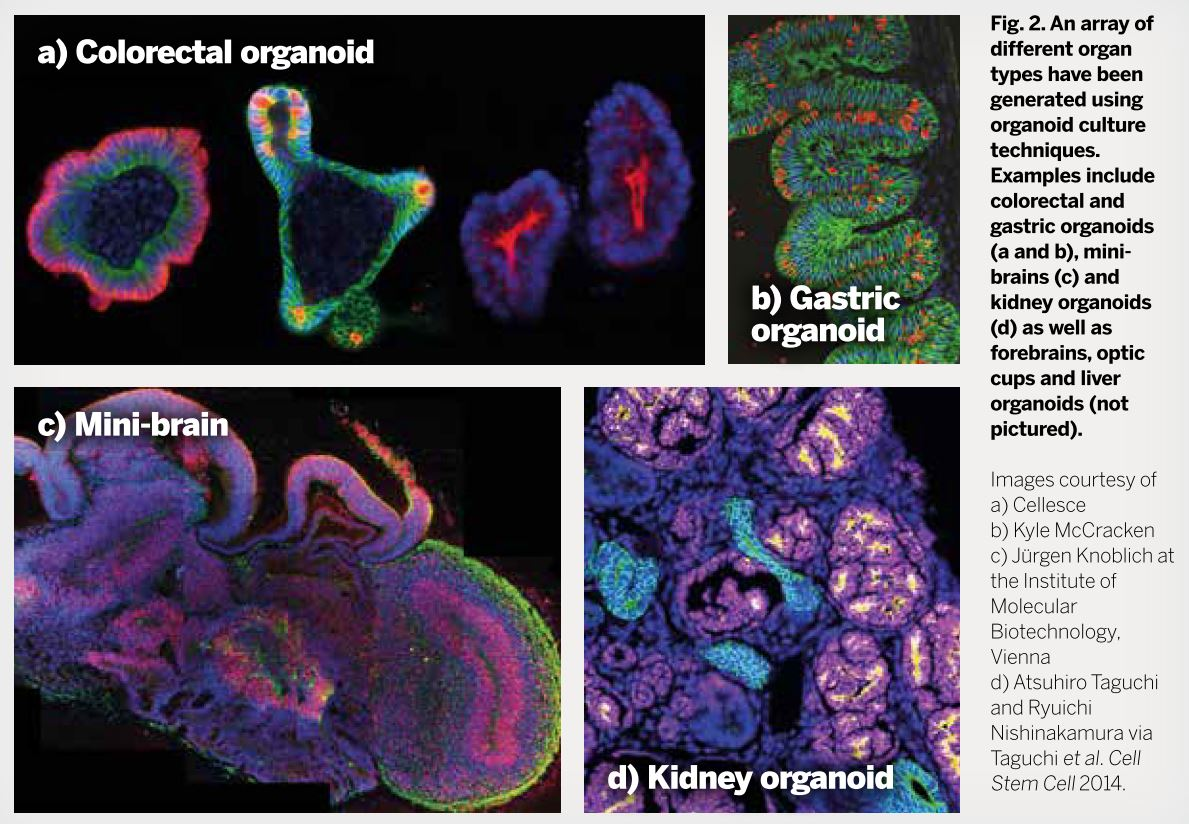
\includegraphics[width=0.65\textwidth]{figures/picture-organoids.jpg}
    \caption{Organoids reproducing different organs. Adapted from \cite{Turner_2020}.}
    \label{fig:pic-organoids}
\end{figure}

In particular, recent studies have succeeded into recapitulating gastrulation, the early stage of embryonic development in which the embryo transforms into a multilayered structure. Such organoid models are known as gastruloids (see Fi\-gure \ref{fig:pic-gastruloid}) \parencite{Brink_2014,Simunovic_2017}.  These or\-ga\-noids form structures similar to those unique to mammalian embryos that define the body axis, and further research is expected to reveal yet unknown mechanisms of development \parencite{Turner_2020}.

\vspace{1em}

\begin{figure}[hb]
    \centering
    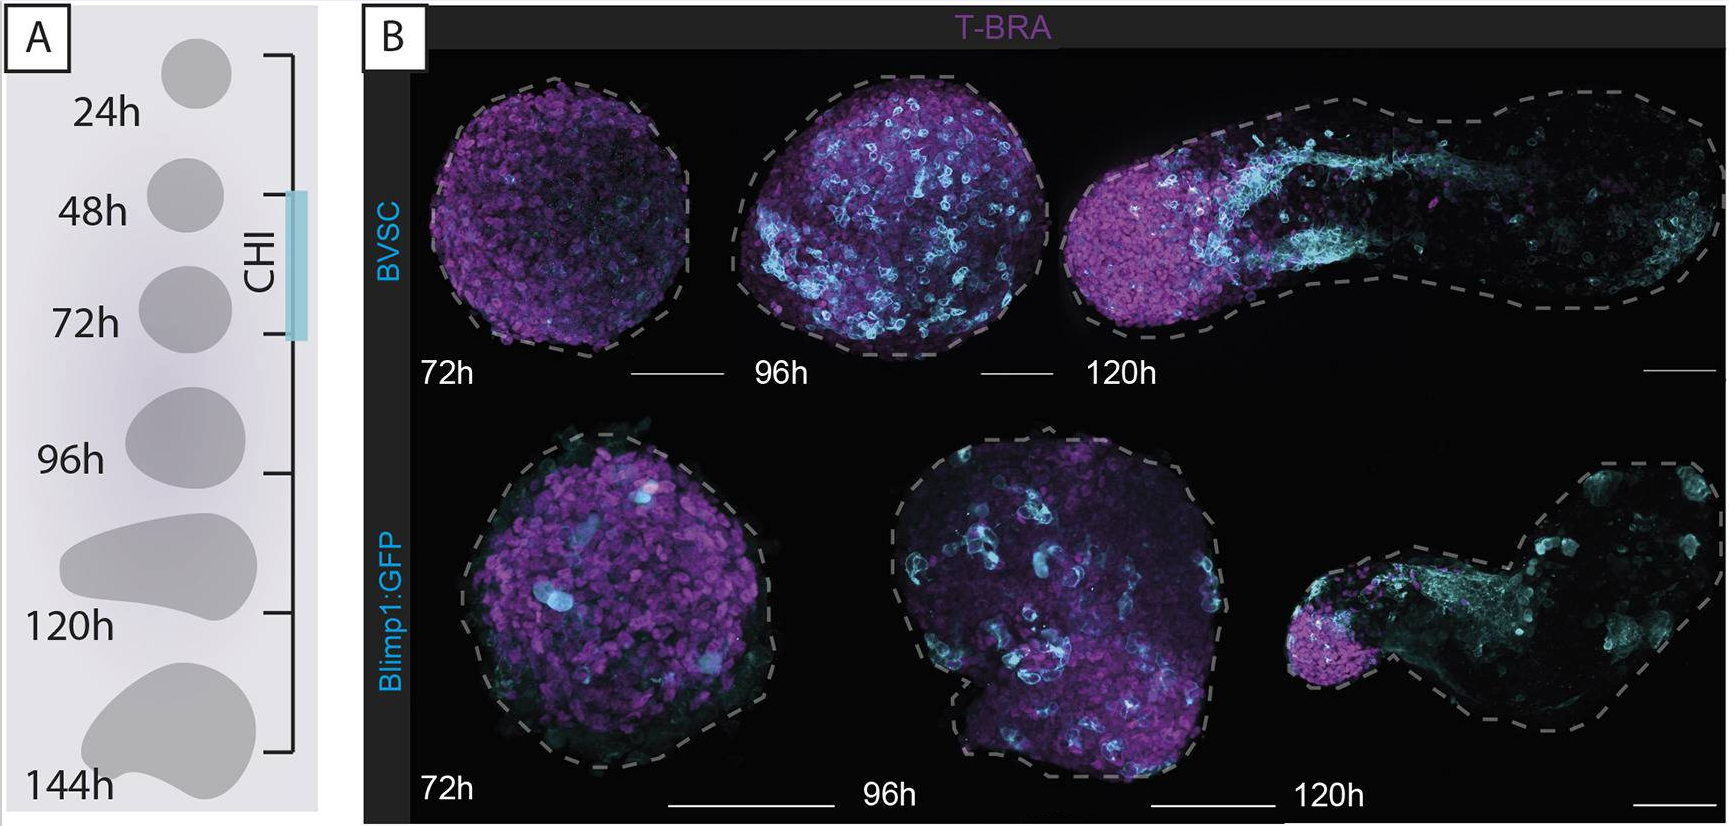
\includegraphics[width=0.7\textwidth]{figures/picture-gastruloid.png}
    \caption{Morphological changes of a gastruloid over time, using markers for different cell states. Adapted from \cite{Cooke_2023}.}
    \label{fig:pic-gastruloid}
\end{figure}



\section{Modelling of organoids}

During embryogenesis, cells communicate and self-organize to form multice\-llular structures, and cell behaviour arises from both physical and chemical in\-te\-rac\-tions (see Fig \ref{fig:pic-embryonic-development}). On the one hand, adhesion, repulsion, and attractive forces influence cell movement. On the other hand, cell-cell signalling drives cell di\-ffe\-ren\-tia\-tion, which in turn affects cell motion. Experimental setups for or\-ga\-noid generation typically involve culturing cells in small volumes under controlled conditions that allow for the monitoring of variables such as cell proliferation, differentiation, and movement. 

One of the key aspects in embryonic development is how the embryo breaks symmetry to form the different body axes. Recent work using the gastruloid system suggests that the timing of this process is controlled by cell-cell communication, and depends on the initial proportions of different type of cells \linebreak \parencite{Oriola_2025}. We aim to construct a model that si\-mu\-lates the early stages of 3D gastruloid development in order to ana\-lyse cell proportions and differentiation kinetics.

\vspace{1em}

\begin{figure}[h]
    \centering
    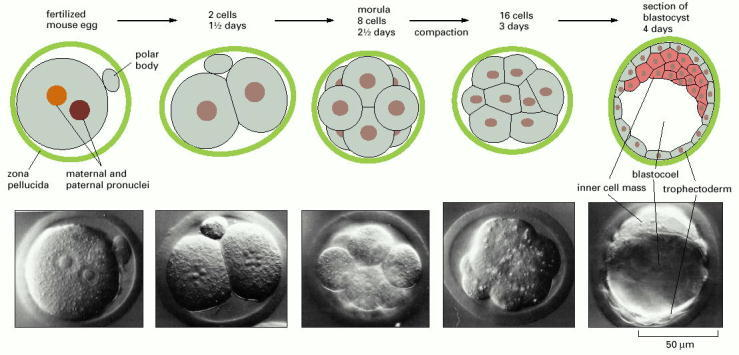
\includegraphics[width=0.75\textwidth]{figures/picture-embryogenesis.jpg}
    \caption{Early stages of mouse embryonic development. Adapted from \cite{Alberts_2002}.}
    \label{fig:pic-embryonic-development}
\end{figure}

Computational models make it possible to study the interplay between cell mechanics and cell signalling. Depending on the focus of analysis, organoid mo\-dels are divided into two main categories: continuum models and agent-based models (ABMs). The former describe tissues as a whole using partial differential equations, while ABMs represent tissue dynamics as the interplay of individual agents \parencite{Liedekerke_2015}.

In this study, we will focus on centre-based models, representing agents as spheres. Cells can divide, move, and interact with other cells, with their motion described by a set of equations for each cell based on pairwise forces. This model supports precise tracking of agents, heterogeneity in cell types, a well-defined timescale, and the modelling of cell-cell interactions \parencite{Liedekerke_2015,Gritti_2021}.

Computations are carried out using the Julia \parencite{Julia_2017} package CellBasedModels.jl \parencite{Torregrosa_2025}. Julia is an open \linebreak source dynamic programming language for scientific computing, characterized by its high performance and attainable reproducibility. The CellBasedModels.jl package offers an understandable and efficient framework for the fast simulation of multicellular communities, allowing mechanical and biochemical interactions to be modelled.



\section{Structure of the thesis}

Expanding on the work of \cite{Liedekerke_2015}, \cite{Saiz_2020}, and \cite{Torregrosa_2023}, we develop and implement a model that aims to si\-mu\-late gastruloids by coupling mechanical interactions and cell fate decisions within a stochastic framework. In Chapter \ref{ch:2-abm}, we present the mathematical model, describing cell mechanics and cell differentiation. In Chapter \ref{ch:3-implementation}, we review the methods used to implement the model, discussing key simplifications necessary for numerical stability. Finally, Chapter \ref{ch:4-applications} presents the applications and analyses performed using the simulation motivated by the results presented in \cite{Oriola_2025}. The \hyperref[ch:appendix]{Appendix} includes mathematical derivations, brief descriptions of the programs used, and supplementary figures.

The primary aim of this work is to design an agent-based model that simulates stable 3D multicellular aggregates, providing clear explanations behind each choice in the model, and to contribute to the scientific community by expanding the documentation for the CellBasedModels.jl package.

All the code developed for this project is available on the \href{https://github.com/MPoLS-lab/villegas-morral-msc-thesis}{Multiscale Physics of Living Systems Group's GitHub \footnote{https://github.com/MPoLS-lab/villegas-morral-msc-thesis}} and on my \href{https://github.com/villegas-morral/masters-thesis}{personal GitHub} \footnote{https://github.com/villegas-morral/masters-thesis}.